\documentclass{article}
\usepackage[utf8]{inputenc}
\usepackage{polski}
\usepackage{geometry}
\usepackage{pdfpages}
\usepackage{pdfpages}
\usepackage{listings}
\usepackage{listingsutf8}
\usepackage{multirow}
\usepackage{siunitx}
\usepackage{multirow}
\usepackage{booktabs}
\usepackage{tabularx}
\usepackage{placeins}
\usepackage{pdflscape}

\geometry{
a4paper,
total={170mm,257mm},
left=20mm,
top=20mm
}
\newcolumntype{Y}{>{\centering\arraybackslash}X}
% \renewcommand\thesection{}
\lstset{%
literate=%
 {ą}{{\k{a}}}1
 {ę}{{\k{e}}}1
 {Ą}{{\k{A}}}1
 {Ę}{{\k{E}}}1
 {ś}{{\'{s}}}1
 {Ś}{{\'{S}}}1
 {ź}{{\'{z}}}1
 {Ź}{{\'{Z}}}1
 {ń}{{\'{n}}}1
 {Ń}{{\'{N}}}1
 {ć}{{\'{c}}}1
 {Ć}{{\'{C}}}1
 {ó}{{\'{o}}}1
 {Ó}{{\'{O}}}1
 {ż}{{\.{z}}}1
 {Ż}{{\.{Z}}}1
 {ł}{{\l{}}}1
 {Ł}{{\l{}}}1
}

\title{Technika Cyfrowa\\
Sprawozdanie - bramki logiczne}
\author{Maciej Trątnowiecki}
\date{AGH, Semestr Letni, 2020}

\begin{document}
    \maketitle
    \section{Układ sumujący dwie liczby trzybitowe}
        \subsection{Projekt układu}
            \begin{center}
                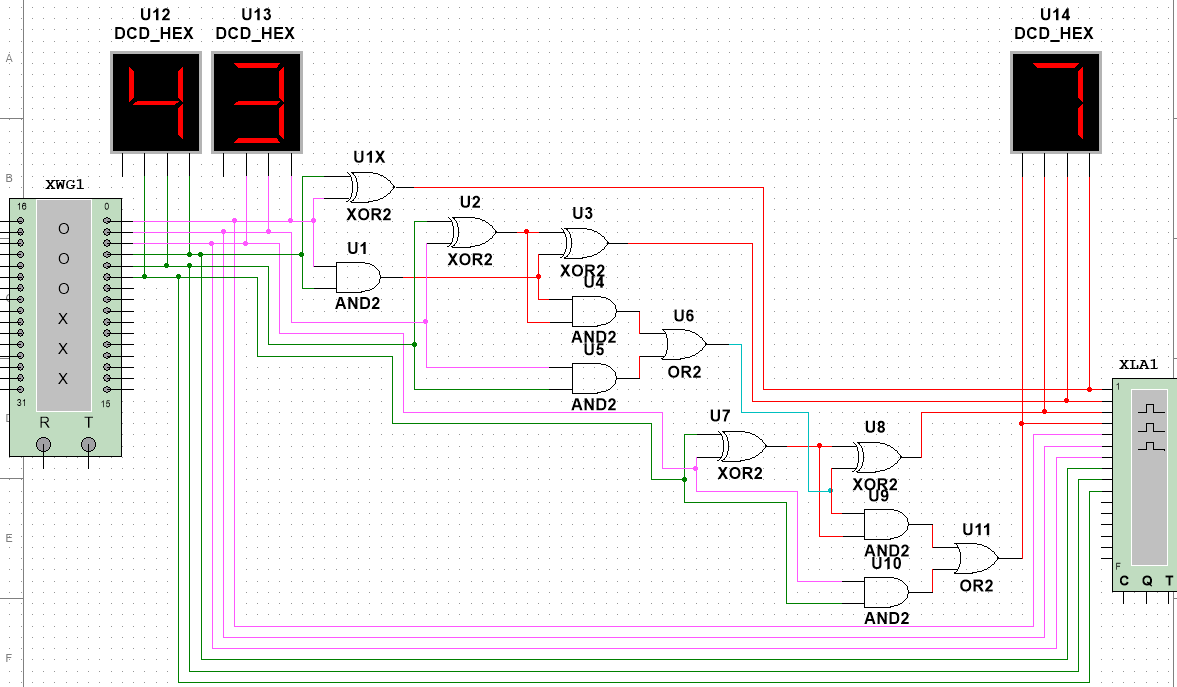
\includegraphics[height=9cm]{reports/img/Z1A_1.png}\\
            \end{center}
            W układzie jako źródło sygnału wykorzystano generator słów. Wyjścia odpowiadające za bity pierwszej z liczb oznaczono kolorem zielonym, a za bity drugiej z nich kolorem różowym. \\
            Do obliczenia sumy arytmetycznej wykorzystano jeden sumator pół-pełny (dla sumy najmniej ważnych bitów), oraz dwa sumatory pełne. Wyjścia odpowiadające za przepełnienie oznaczono kolorem lazurowym. \\
            Wynik operacji zilustrowano poprzez wykorzystanie wyświetlacza HEX. 
    \section{Układ sprawdzający równość dwóch liczb}
        \subsection{Projekt układu}
            \begin{center}
                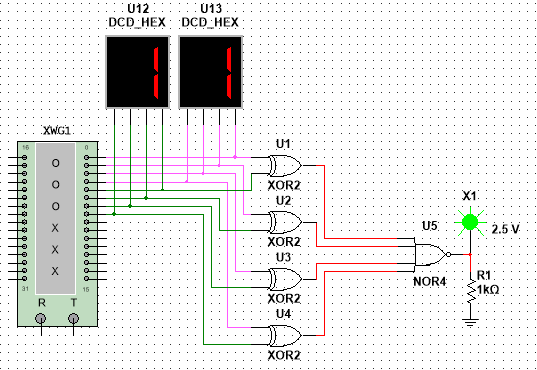
\includegraphics[height=9cm]{reports/img/Z1B_1.png}\\
            \end{center}
            W układzie jako źródło sygnału wykorzystano generator słów. Wyjścia odpowiadające za bity pierwszej z liczb oznaczono kolorem zielonym, a za bity drugiej z nich kolorem różowym. \\
            Do porównania wartości liczb wykorzystano bramki xor, których wyniki zbiera bramka nor. \\
            Równość liczb sygnalizuje zielona dioda. 

    \section{Transkoder czterobitowych cyfr szesnastkowych na wyświetlacz siedmiosegmentowy}
        \subsection{Minimalizacja funkcji boolowskich}
            Wyświetlaczem sterować można poprzez 7 wyjść, ponumerowanych od A do G, każde z nich odpowiada za inny segment wyświetlacza. W poniższej tabeli zebrano opis ustawień wyjść odpowiedzialnych za wyświetlanie każdej z liczb czterobitowych.
            \begin{center}
                \begin{table}[ht]
                    \centering
                    \begin{tabularx}{\textwidth}{|c|c| *{7}{Y|}} %{|c|c|c|c|c|c|c|c|c|}
                        \hline
                        % \multirow{ 2}{*}{Liczba w systemie szesnastkowym} &  
                        % \multirow{ 2}{*}{Liczba w systemie binarnym} &
                        \textbf{Liczba w systemie} & \textbf{Liczba w systemie} &
                        \multicolumn{7}{|l|}{\textbf{Wyjścia wyświetlacza siedmiosegmentowego}}\\
                        \cline{3-9}
                        \textbf{szesnastkowym} & \textbf{binarnym} & \textbf{A} & \textbf{B} & \textbf{C} & \textbf{D} & \textbf{E} & \textbf{F} & \textbf{G} \\
                        \specialrule{.1em}{.05em}{.05em} 
                         0 & 0000 & 0 & 0 & 0 & 0 & 0 & 0 & 0\\
                         \hline 
                         1 & 0001 & 0 & 1 & 1 & 0 & 0 & 0 & 0\\
                         \hline 
                         2 & 0010 & 1 & 1 & 0 & 1 & 1 & 0 & 1\\
                         \hline 
                         3 & 0011 & 1 & 1 & 1 & 1 & 0 & 0 & 1\\
                         \hline 
                         4 & 0100 & 1 & 1 & 1 & 0 & 0 & 1 & 1\\
                         \hline 
                         5 & 0101 & 1 & 0 & 1 & 1 & 0 & 1 & 1\\
                         \hline 
                         6 & 0110 & 1 & 0 & 1 & 1 & 1 & 1 & 1\\
                         \hline 
                         7 & 0111 & 1 & 1 & 1 & 0 & 0 & 0 & 0\\
                         \hline 
                         8 & 1000 & 1 & 1 & 1 & 1 & 1 & 1 & 1\\
                         \hline 
                         9 & 1001 & 1 & 1 & 1 & 0 & 0 & 1 & 1\\
                         \hline
                         A & 1010 & 1 & 1 & 1 & 0 & 1 & 1 & 1\\
                         \hline
                         B & 1011 & 0 & 0 & 1 & 1 & 1 & 1 & 1\\ 
                         \hline
                         C & 1100 & 1 & 0 & 0 & 1 & 1 & 1 & 0\\
                         \hline
                         D & 1101 & 0 & 1 & 1 & 1 & 1 & 0 & 1\\
                         \hline
                         E & 1110 & 1 & 0 & 0 & 1 & 1 & 1 & 1\\
                         \hline
                         F & 1111 & 1 & 0 & 0 & 0 & 1 & 1 & 1\\
                        \hline
                    \end{tabularx}
                    \caption{Wyjścia wyświetlacza}
                    \label{tab:my_label}
                \end{table}
            \end{center}
            \FloatBarrier
            
            W celu uproszczenia układu wykonać należy minimalizację metodą Karnaugh dla każdego z wyjść wyświetlacza. Niech $x_1, x_2, x_4, x_8$ określają kolejne bity, czterobitowej liczby $x$ w kolejności od najmniej do najbardziej znaczącego bitu. Wtedy:
            \begin{center}
                \begin{table}[ht]
                    \centering
                    \begin{tabularx}{\textwidth}{|Y *{5}{Y|}}
                        \cline{3-6} 
                        \multicolumn{2}{c|}{} &
                        \multicolumn{4}{c|}{$x_1x_2$}\\
                        
                        \multicolumn{2}{c|}{} & \multicolumn{1}{c}{00} & \multicolumn{1}{c}{01} & \multicolumn{1}{c}{11} & \multicolumn{1}{c|}{10}\\
                        \hline
                         
                        \multirow{4}{*}{$x_4x_8$} & 00 & 0 & 0 & 1 & 1 \\
                                                  & 01 & 0 & 1 & 0 & 1 \\
                                                  & 11 & 1 & 1 & 1 & 0 \\
                                                  & 10 & 1 & 1 & 1 & 1 \\
                        
                         \hline 
                    \end{tabularx}
                    \caption{Wyjście A}
                    \label{tab:my_label}
                \end{table}
            \end{center}
            \FloatBarrier
            Skąd otrzymujemy (przez dopełnienie):
            $$A = (x_4+x_1+x_2)(x_1+x_4+x_8)(x_4+\overline{x_8}+\overline{x_1}+\overline{x_2})(x_2+\overline{x_1}+\overline{x_4}+\overline{x_8})$$
            
            \begin{center}
                \begin{table}[ht]
                    \centering
                    \begin{tabularx}{\textwidth}{|Y *{5}{Y|}}
                        \cline{3-6} 
                        \multicolumn{2}{c|}{} &
                        \multicolumn{4}{c|}{$x_1x_2$}\\
                        
                        \multicolumn{2}{c|}{} & \multicolumn{1}{c}{00} & \multicolumn{1}{c}{01} & \multicolumn{1}{c}{11} & \multicolumn{1}{c|}{10}\\
                        \hline
                         
                        \multirow{4}{*}{$x_4x_8$} & 00 & 0 & 0 & 1 & 1 \\
                                                  & 01 & 1 & 1 & 0 & 1 \\
                                                  & 11 & 1 & 1 & 1 & 0 \\
                                                  & 10 & 1 & 1 & 1 & 1 \\
                        
                         \hline 
                    \end{tabularx}
                    \caption{Wyjście B}
                    \label{tab:my_label}
                \end{table}
            \end{center}
            \FloatBarrier
            Skąd otrzymujemy (przez dopełnienie):
            $$ B = (x_1+x_4+x_8)(\overline{x_1}+\overline{x_2}+x_4+\overline{x_8})(\overline{x_1}+x_2+\overline{x_4}+\overline{x_8})$$
            
            \begin{center}
                \begin{table}[ht]
                    \centering
                    \begin{tabularx}{\textwidth}{|Y *{5}{Y|}}
                        \cline{3-6} 
                        \multicolumn{2}{c|}{} &
                        \multicolumn{4}{c|}{$x_1x_2$}\\
                        
                        \multicolumn{2}{c|}{} & \multicolumn{1}{c}{00} & \multicolumn{1}{c}{01} & \multicolumn{1}{c}{11} & \multicolumn{1}{c|}{10}\\
                        \hline
                         
                        \multirow{4}{*}{$x_4x_8$} & 00 & 0 & 1 & 0 & 1 \\
                                                  & 01 & 1 & 1 & 1 & 1 \\
                                                  & 11 & 1 & 1 & 0 & 1 \\
                                                  & 10 & 0 & 1 & 0 & 1 \\
                        
                         \hline 
                    \end{tabularx}
                    \caption{Wyjście C}
                    \label{tab:my_label}
                \end{table}
            \end{center}
            \FloatBarrier
            Skąd otrzymujemy (przez dopełnienie):
            $$C = (x_1+x_2+x_8)(\overline{x_1}+\overline{x_2}+\overline{x_4})(\overline{x_1}+\overline{x_2}+x_4+x_8)$$
            
            \begin{center}
                \begin{table}[ht]
                    \centering
                    \begin{tabularx}{\textwidth}{|Y *{5}{Y|}}
                        \cline{3-6} 
                        \multicolumn{2}{c|}{} &
                        \multicolumn{4}{c|}{$x_1x_2$}\\
                        
                        \multicolumn{2}{c|}{} & \multicolumn{1}{c}{00} & \multicolumn{1}{c}{01} & \multicolumn{1}{c}{11} & \multicolumn{1}{c|}{10}\\
                        \hline
                         
                        \multirow{4}{*}{$x_4x_8$} & 00 & 0 & 0 & 1 & 1 \\
                                                  & 01 & 0 & 1 & 1 & 0 \\
                                                  & 11 & 1 & 0 & 0 & 1 \\
                                                  & 10 & 1 & 1 & 1 & 0 \\
                        
                         \hline 
                    \end{tabularx}
                    \caption{Wyjście D}
                    \label{tab:my_label}
                \end{table}
            \end{center}
            \FloatBarrier
            Skąd otrzymujemy (przez dopełnienie):
            $$D = (x_1+x_4+x_8)(\overline{x_2}+\overline{x_4}+\overline{x_8})(x_2+x_4+\overline{x_8})(\overline{x_1}+x_2+\overline{x_4}+x_8)$$
        
            \begin{center}
                \begin{table}[ht]
                    \centering
                    \begin{tabularx}{\textwidth}{|Y *{5}{Y|}}
                        \cline{3-6} 
                        \multicolumn{2}{c|}{} &
                        \multicolumn{4}{c|}{$x_1x_2$}\\
                        
                        \multicolumn{2}{c|}{} & \multicolumn{1}{c}{00} & \multicolumn{1}{c}{01} & \multicolumn{1}{c}{11} & \multicolumn{1}{c|}{10}\\
                        \hline
                         
                        \multirow{4}{*}{$x_4x_8$} & 00 & 0 & 0 & 1 & 1 \\
                                                  & 01 & 0 & 0 & 1 & 0 \\
                                                  & 11 & 0 & 0 & 1 & 1 \\
                                                  & 10 & 1 & 1 & 1 & 1 \\
                        
                         \hline 
                    \end{tabularx}
                    \caption{Wyjście E}
                    \label{tab:my_label}
                \end{table}
            \end{center}
            \FloatBarrier
            Skąd otrzymujemy (przez dopełnienie):
            $$E = (x_1+x_4)(x_1+\overline{x_4}+\overline{x_8})(\overline{x_1}+x_2+x_4+\overline{x_8})$$
            
            \begin{center}
                \begin{table}[ht]
                    \centering
                    \begin{tabularx}{\textwidth}{|Y *{5}{Y|}}
                        \cline{3-6} 
                        \multicolumn{2}{c|}{} &
                        \multicolumn{4}{c|}{$x_1x_2$}\\
                        
                        \multicolumn{2}{c|}{} & \multicolumn{1}{c}{00} & \multicolumn{1}{c}{01} & \multicolumn{1}{c}{11} & \multicolumn{1}{c|}{10}\\
                        \hline
                         
                        \multirow{4}{*}{$x_4x_8$} & 00 & 0 & 1 & 1 & 1 \\
                                                  & 01 & 0 & 1 & 1 & 0 \\
                                                  & 11 & 0 & 0 & 1 & 1 \\
                                                  & 10 & 0 & 1 & 1 & 1 \\
                        
                         \hline 
                    \end{tabularx}
                    \caption{Wyjście F}
                    \label{tab:my_label}
                \end{table}
            \end{center}
            \FloatBarrier
            Skąd otrzymujemy (przez dopełnienie):
            $$F = (x_1+x_2)(x_1+\overline{x_2}+\overline{x_4}+\overline{x_8})(\overline{x_1}+x_2+x_4+\overline{x_8})$$

            
            \begin{center}
                \begin{table}[ht]
                    \centering
                    \begin{tabularx}{\textwidth}{|Y *{5}{Y|}}
                        \cline{3-6} 
                        \multicolumn{2}{c|}{} &
                        \multicolumn{4}{c|}{$x_1x_2$}\\
                        
                        \multicolumn{2}{c|}{} & \multicolumn{1}{c}{00} & \multicolumn{1}{c}{01} & \multicolumn{1}{c}{11} & \multicolumn{1}{c|}{10}\\
                        \hline
                         
                        \multirow{4}{*}{$x_4x_8$} & 00 & 0 & 1 & 1 & 0 \\
                                                  & 01 & 0 & 1 & 1 & 1 \\
                                                  & 11 & 1 & 0 & 1 & 1 \\
                                                  & 10 & 1 & 1 & 1 & 1 \\
                        
                         \hline 
                    \end{tabularx}
                    \caption{Wyjście G}
                    \label{tab:my_label}
                \end{table}
            \end{center}
            \FloatBarrier
            Skąd otrzymujemy (przez dopełnienie):
            $$G = (x_1+x_2+x_4)(\overline{x_1}+x_2+x_4+x_8)(x_1+\overline{x_2}+\overline{x_4}+\overline{x_8})$$
            
\end{document}
